\RequirePackage[hyphens]{url}

\documentclass[sigconf]{acmart}

\usepackage{graphicx}
\usepackage{hyperref}
\usepackage{todonotes}

\usepackage{endfloat}
\renewcommand{\efloatseparator}{\mbox{}} % no new page between figures

\usepackage{booktabs} % For formal tables

\settopmatter{printacmref=false} % Removes citation information below abstract
\renewcommand\footnotetextcopyrightpermission[1]{} % removes footnote with conference information in first column
\pagestyle{plain} % removes running headers

\newcommand{\TODO}[1]{\todo[inline]{#1}}

\begin{document}
\title{Big data and hearing disability}


\author{Rahul Velayutham}
\affiliation{%
  \institution{Indiana University Bloomington}
  \streetaddress{2661 H 7th St}
  \city{Bloomington} 
  \state{Indiana} 
  \postcode{47408}
}
\email{rahuvela@umail.iu.edu}

% The default list of authors is too long for headers}
\renewcommand{\shortauthors}{R. Velayutham}


\begin{abstract}
Big Data is rapidly becoming a crucial component in the majority of the fields, be it from medicine to software. Big data technologies help in processing humongous amounts of data in a rapid manner while enabling us to achieve results fast and accurately. Hearing disability is a huge problem to the very fabric of society. It causes great discomfort among those who suffer from it and in some extreme cases can cause alienation. Thus there is a need for society to accept the difficulties faced by those are affected with hearing disabilities and enhance the traditional solutions offered with the latest technologies so that they can lead a life without difficulties and live a normal life. The paper shows how the latest big data trends can be applied to existing traditional solutions like hearing aid , captions and also suggests how it can used to proactively avoid situations that could lead to hearing loss. It is hoped that an interest will be generated towards further reserach and implementaion towards combining Big data with hearing difficulty solutions.
\end{abstract}

\keywords{Big Data, i523 , HID 232 , Rain Water Harvesting}


\maketitle



\section{Introduction}

Hearing loss or impairment is defined as the partial or total inability to hear and may occur in one or both ears and may result in a person having little to no hearing. This loss can be either temporary or permanent depending on the mode of affliction. The causes of hearing loss are many but the most prominent factors can be narrowed down to genetics, ageing, exposure to noise, some infections, birth complications, trauma to the ear, and certain medications or toxins, chronic ear infections and the ilk. Infections that may no relation to hearing loss like syphilis and rubella may also cause hearing loss if infected during pregnancy. If a person feels that their hearing is not sharp they can undergo tests to confirm which sets the bar at 25 decibels, if a person cant hears at that range then they can be diagnosed as suffering from hearing loss. Hearing loss can be categorized as mild, moderate, moderate-severe, severe, or profound\cite{Wikipedia2017}. Hearing loss can further be categorized into two sections Congenital Hearing Loss and Acquired Hearing Loss.Under Congenital Hearing Loss two chief factors are Genetic and Prenatal Issues. Under Acquired Hearing Loss the chief factors can be listed as Chronic ear infections, medications that can affect aspects of hearing, Diseases that affect hearing (Ménière's Disease, etc.), Head injury, Perforated eardrum\cite{Academy2017}.

Generally, genetic factors have been found to be responsible for pediatric hearing loss. This occurs when inherited genes work against the development of the patient's body and this impacts the development of the hearing system as a result. As it is with genetics it can target any to every part of the body in this case it spares no part of the ear and can target any part from the outer ear to the deepest part of the inner ear. The degree of hearing loss can vary depending on which part is affected. When applicable solutions like hearing aids, implants etc provide for some relief \cite{Wikipedia2017}.

As of 2013 hearing loss affects about 1.1 billion people to some degree\cite{Wikipedia2017}.It causes disability in 5\% (360 to 538 million) and moderate to severe disability in 124 million people \cite{Wikipedia2017} . Of those with moderate to severe disability 108 million live in low and middle-income countries.Of those with hearing loss, it began in 65 million during childhood.Those who use sign language and are members of Deaf culture see themselves as having a difference rather than an illness.Most members of Deaf culture oppose attempts to cure deafness and some within this community view cochlear implants with concern as they have the potential to eliminate their culture.The term hearing impairment is often viewed negatively as it emphasizes what people cannot do. Despite all of the solutions and rationalizations being made, it cannot be denied however that hearing loss is becoming an important problem in today's society and one whose numbers is constantly increasing\cite{Wikipedia2017}.

Big data is the perhaps the most interesting technological advancement made in the current era, it has roots in almost all fields right from health care to education to even government policies. It is the far reach that makes big data important, it allows users and clients to make better-informed decisions by taking into account almost all factors. doctors are looking towards big data to make more accurate diagnostics and look for new medicines, economists are looking towards big data to make more accurate models. The paper will look into how it can enhance some of the solutions provided for those hard of hearing like hearing aids, closed caption etc. It will also suggest enhancements towards preemptively preventing situations that could lead to hearing loss\cite{Wikipedia2017}.

\section{big data in hearing aids}

\subsection{Introduction}


Hearing aids are small electronic devices that you wear in or behind your ear they improve the hearing and speech comprehension of people. It makes some sounds louder so that a person with hearing loss can listen, communicate, and participate more fully in daily activities. A hearing aid can help people hear more in both quiet and noisy situations. A hearing aid has three basic parts: a microphone, amplifier, and speaker as can be seen from the figure \ref{f:hearingaidparts}.

\begin{figure}[!ht]
  \centering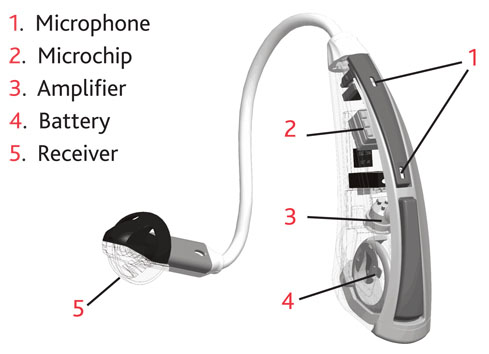
\includegraphics[width=\columnwidth]{images/hearingaidbreakdown.jpg}
  \caption{parts of hearing aid}\label{f:hearingaidparts}
\end{figure}  

The microphone receives sound, which converts it into electrical signals and sends them to an amplifier. The amplifier increases the power of the signals and then sends them to the ear through a speaker basically it is magnifying sound vibrations entering the ear. The eardrum then passes these vibrations to the nerve cells which then passes these signals to the brain. The more severe the hearing loss, and the greater the hearing aid amplification needed to make up the difference. However, there are practical limits to the amount of amplification a hearing aid can provide. However, if the inner ear is too damaged, a hearing aid would be ineffective \cite{NIHCD2017}.
\newline
Hearing aids can be classified into three distinct categories \cite{NIHCD2017} they are Behind-the-ear (BTE), In-the-ear (ITE) and Canal as can be seen in the figure \ref{f:typesofaids}.  
\begin{figure}[!ht]
  \centering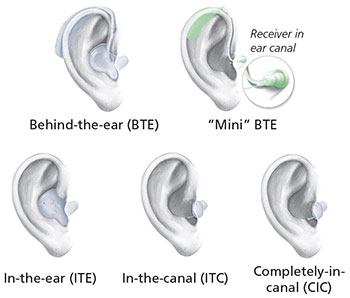
\includegraphics[width=\columnwidth]{images/typesofaids.jpg}
  \caption{types of hearing aids}\label{f:typesofaids}
\end{figure}  
BTE hearing aids consist of a hard plastic case worn behind the ear and connected to a plastic earmold that fits inside the outer ear. The electronic parts are held in the case behind the ear. Sound travels from the hearing aid through the earmold and into the ear. BTE aids are used by people of all ages for mild to profound hearing loss. ITE aids fit completely inside the outer ear and are used for mild to severe hearing loss. The case holding the electronic components is made of hard plastic.  Canal Aids fit into the ear canal and are available in two styles. The in-the-canal (ITC) hearing aid is made to fit the size and shape of a person’s ear canal. A completely-in-canal (CIC) hearing aid is nearly hidden in the ear canal. Both types are used for mild to moderately severe hearing loss\cite{NIHCD2017}.
\newline
Hearing aids can further be classified based on their inner circuitry which is analogue and digital.Analog aids convert sound waves into electrical signals, which are amplified. The aid is programmed by the manufacturer according to the specifications recommended by your audiologist. An audiologist can program the aid using a computer, and you can change the program for different listening environments from a small, quiet room to a crowded restaurant etc.Digital aids convert sound waves into numerical codes, similar to the binary code of a computer, before amplifying them. Because the code also includes information about a sound’s pitch or loudness, the aid can be specially programmed to amplify some frequencies more than others. Digital circuitry gives an audiologist more flexibility in adjusting the aid to a user’s needs and to certain listening environments and can be programmed to focus on sounds coming from a specific direction\cite{NIHCD2017}.

Hearing aids are a fairly popular solution among most age groups and users use them for about 8-9 hours a day \cite{Audiol.2017}.The process of getting a hearing aid is fairly simple. First, you confirm with an ENT / audiologist that you are indeed in need of one. Then a series of audiometery tests are performed to determine the extent of damage / hearing loss incurred. Hearing sensitivity can be measured for a range of frequencies and plotted on an audiogram. Another method for quantifying hearing loss is a speech-in-noise test, which gives an indication of how well one can understand speech in a noisy environment. A person with a hearing loss will often be less able to understand speech, especially in noisy conditions. This is especially true for people who have a sensorineural loss – which is by far the most common type of hearing loss.  A recently developed digit-triple speech-in-noise test may be a more efficient screening test.The audiologist then programs the hearing aid to amplify at an acceptable level.


\subsection{Big data in hearing aids}

The working of hearing aids was covered in detail in the previous section now we shall focus on the areas where big data can be applied to help both the doctors and the patients as much as possible. We know that in order to determine the extent of hearing loss an audiometry test will be performed. The test proceeds with a patient being made to sit in a soundproof room and being subjected to listening to a wide variety of sounds ranging from the softest possible sound they can perceive to the loudest possible. The audiologist then charts a graph to figure out the extent of hearing loss. It will look like the below graph shown as per the figure  \ref{f:audiometrygraph}.
\begin{figure}[!ht]
  \centering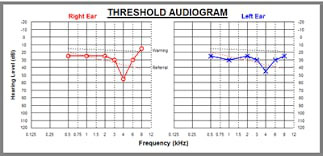
\includegraphics[width=\columnwidth]{images/audiometerygraph.jpg}
  \caption{audiometry graph}\label{f:audiometrygraph}
\end{figure}  
The problem with this process is it's still random and despite audiologists having great skill and lowering the margin as much as possible they can never be totally accurate nor can they test too much because it is physically demanding on the patient too. Big data can be a great help here. Data collected from multiple patients (with their consent) can be stored making use of technologies like apache pig , hive etc. Then when an initial audiometry analysis has been performed we can use deep learning or simple statistical sampling to obtain a few similar cases via technologies like say apache-spark. From these cases, we can perform a more streamlined audiometry test rather than guesswork and further accurately narrow down the loss coefficients. 
\newline
After the hearing loss estimates are charted down. It is time to program the hearing aid (a hearing aid model is selected by the audiologist in accordance with the hearing loss estimates). The aid is programmed to amplify sound waves in the range where losses are observed and then various simulated environments are performed to determine the level of comfort and extent to which the hearing aid is helping and perform fine-tuning.The problem is the same as previous a very limited range of environment that may / may not be useful to the patient is observed. Using big data once again a more accurate test can be conceived. A user can be presented with the environments patients from the similar range of hearing loss faced and this can be used as a basis for fine-tuning. This process has slowly been making its way into research \cite{peternordquist2017} and a few companies \cite{phonak2017} have already started commercialising it.
\newline
 These days most people make use of digital hearing aids. As previously mentioned digital hearing aids are well equipped to make use of big data in a way they do make use of it albeit in a micro manner. The behavioural patterns of the patient are recorded like the range of volume increase or decrease in various modes, amount used etc. When the patient visits the audiologist the next time this data is analysed and then corrective changes are made towards the programming of the hearing aid. Big data can play a very big role in proactively doing so. These days most hearing aids have moved on from using a separate remote control towards making use of smartphone apps as a remote. This can be viewed as a huge enabler for big data technologies. Since mobile phones will most of the time be connected to the internet this will enable (with consent) real-time load and store of data using technologies like pig and hadoop of user environments and the current sound wave patterns and amplification used along with other useful data like if the patient is increasing or decreasing volume. Hearing aids are certainly growing smarter in the sense when a mobile communication device is brought near the aid the electromagnetic pulses from the phone is detected by the aid and automatically switches to a phone mode, however for most of the part the user has to switch manually to other modes like theatre, noisy etc. Big data can play a huge role in automatic detection. For starters, big data can be employed to dynamically observe the fluctuations in loudness levels as well observe the fluctuations in background noise to help determine what mode should aid change to. Aise from observing fluctuations it can also compare the current scenario to those who have already encountered such scenarios under similar conditions ( and with a similar hearing loss) rate and then perhaps adjust the volume/setting to a safe appropriate level. note that this would be highly experimental and could also create more problems than it solves. As much as we have powerful machine learning algorithms like deep learning it is impossible for them to predict a solution that best suits a patient after all different patients have different problems and conditions but as it learns more and gains more data (the hallmark of deep learning to learn with more data) there will be a good chance that the algorithms will  provide a solution that really suits the patient.
 \newline
So far we have looked at how big data can make use of sound waves in terms of loudness background noise etc, but there is one more aspect in which big data can help us. Analysing the contents of the speech itself.It has been previously mentioned Big data in language and speech processing is a well-established topic and plenty of papers and discussions exists \cite{Chung2017} \cite{Schuller2015}. Most speech can be well predicted these days and when we take into account that hearing aids these days can make out the direction of which the sound is coming from. Making use of this and the ability of deep learning to possibly predicts parts of speech we can leverage this to accordingly increase or decrease volume. certain words will have pronunciations that are hard to understand or have lower tones or have a high frequency to be repeated. we can take advantage of this. Also, the hearing aid can be programmed to automatically increase the volume when it detects a repetition of sentences/words either due to the patient asking the opposite person to repeat his/her sentence. this can be achieved either by listening to keywords like what, sorry, repeat yourself, etc or by analysing the sound waves and learning from that if the same pattern is being repeated. 

\subsection{Data processing and Technologies}

 
Pattern recognition is a branch of machine learning that focuses on the recognition of patterns and regularities in data. Pattern recognition systems are in many cases trained from labelled "training" data (supervised learning), but when no labelled data are available other algorithms can be used to discover previously unknown patterns (unsupervised learning).In machine learning, pattern recognition is the assignment of a label to a given input value.An example of pattern recognition is classification, which attempts to assign each input value to one of a given set of classes (for example, determine whether a given email is "spam" or "non-spam"). However, pattern recognition is a more general problem that encompasses other types of output as well. Other examples are regression, which assigns a real-valued output to each input; sequence labeling, which assigns a class to each member of a sequence of values (for example, part of speech tagging, which assigns a part of speech to each word in an input sentence); and parsing, which assigns a parse tree to an input sentence, describing the syntactic structure of the sentence \cite{2017b}.
\newline
From the above explanation, it becomes clear the manner in which we can apply pattern matching for hearing aids. We could use the binary stream as a basis for calculation and from this stream try to match it to existing patterns and predict the future patterns. If any of the generated patterns are found to have speech that is hard to decipher at that range signals can be sent to the hearing aid to according raise the volume of the hearing aid. Aside from that we can make use of the binary sequences and try to find the best fit pattern match, we can eliminate noise because most hearing aids these days have excellent noise cancelling technology so we can be assured that the sound stream is that of the person who is speaking to the patient. Once we get the best fit we can make a correlation between the pattern identified and the next action to be performed. 
\newline
The discussed methods need not only be limited to merely volume increase and decrease. they can also be applied to the fitting process as we have discussed in detail previously, after obtaining the initial estimate graph we can take the plot points and use it to find the best-fit match of another patient  and fine-tune the hearing aid accordingly saving a lot of time and effort and allowing the entire experience to be pleasant and more productive.
\newline
Apache hadoop, hive etc are just data warehousing software, used for distributed storage and processing of dataset of big data using the MapReduce programming model. It consists of computer clusters built from commodity hardware. All the modules in Hadoop are designed with a fundamental assumption that hardware failures are common occurrences and should be automatically handled by the framework.we have previously seen how data is being made available for us the next logical question that comes to mind is how do we store it and using what. The answer to what is somewhat easier to explain. As mentioned previously we can make use of sound waves which gets converted to numerical codes. Mobile phones used to control the hearing aids which have access to the internet can make use of hadoop framework. We can send this data to some API which then uses map reduce to accordingly save it to a location which represents that pattern. while looking for a pattern the analysis made at real time can be used to query the API which will use map reduce to obtain all patterns relevant to the range of hearing loss and then use pattern matching to figure out best fits and suggest feasible solutions. Audiologists can make use of this in the same manner only instead of making use of the API via mobile phones they can do it conventionally by a computer which will allow for stronger processing.


\subsection{Section Summary}

Hearing aids are the most assistive technology a person with hearing impairments could receive which do not require surgery. They are fast becoming an important industry especially with the rising problem of hearing loss. The process of obtaining a hearing aid is simple and straightforward and for a long time it remained static. However with the advent of big data the world of hearing aids has been shaken from its static foundations and is undergoing a paradigm shift in the same manner mobile phones evolved to the current smart model. Right from the process of fitting to using the hearing big data can be applied to almost every stage. the entire process is still in its infancy and there is a huge scope for further development. Pattern matching , deep learning all the concepts are only the tip of the iceberg there are many algorithms and designs that can Be implemented. Thus there is a huge market both towards improving the current crop of hearing aids available and as well as creating jobs.



\section{Big data in closed captioning}

\subsection{Introduction}

The importance of video in today's world cannot be stated enough. in the field of education, more and more classes are being shifted to the online model, professors are moving towards keeping their lecturers in places like udemy, youtube, pluralsight etc because there they are allowed the total freedom to take the course in their own direction without the constraints of time and classroom size. Certain sites like youtube even offer a source of remuneration. Thanks to the advancements in technology like smartphones and cheaper internet the general public is not satisfied with just listening to the audio, they want to watch the video and embrace the whole experience and artists have contributed to it by making their videos so colourful. TV is ever present with people preferring to watch news comfortably and be updated on the go rather than rifle through a newspaper. Even in communication, there is a paradigm shift from normal audio based conversations heading towards video calls, facetime, Whatsapp video chat are just a few of the most popular options available.
\newline
Now that an accord has been reached on how popular the video format is becoming, its time to talk about how difficult it's becoming for people who have hearing disabilities to cope with this changing world. These are people who are struggling to understand communication face to face and now are tasked with trying to understand something available on a digital platform and something they may not even have the power to ask for a repeat in case they misheard. the problem with digital media is mainly the distortion that comes with it. If it is too loud it becomes illegible to understand if it's too soft it is not loud enough to understand and the middle ground isn't much of a help more often than not. Aside from videos hearing impaired patients also find it difficult to perform most of their daily life activities like attending a class etc.
\newline
So what solution do we have that is capable of solving most of the above problems. It can be observed that the community has gone about finding different ways to solve their problems. Sign language translators, lip reading etc. They are all convenient methods of getting by but the problem with them is as good as they are they are way too situational. A more reliable method would be that of closed captions. Note that the art of captions is one that already exists and is made mandatory by governments to make such resources available on request and in general people are very receptive towards these technologies and often go out of their way to enable them.
For students perhaps the most common use of captions is the CART(Communication Access Real Time) systems, where an individual types a captioning of what the teacher is saying and the students view this in real time there will always be a delay of a few microseconds but it is still extremely useful \cite{Wikipedia2017} . In the case of tv, most channels already have implemented a subtitle system. Pre-recorded shows already have subtitles generated in advance and they are displayed. In case of live settings, the same text from the teleprompter is used as a subtitle or a cart like a system is used where a person types in the text being spoken and it is displayed a few seconds later.In the case of online videos, most content providers have provided the option of loading the subtitle file. The problem now lies in generating/obtaining the subtitle files. Good Samaritans always exist and for important videos more often than not the uploader or someone else will generate their own subtitles. The society is slowly recognizing the need for subtitles and in general, you will find the subtitles of the files you are looking for if you look hard enough. There also exist professional agencies who will create subtitles either for free or for a price, though in general, the free ones are already hard at work. 
\newline
The issue at hand today is generating good quality subtitles and fast. The traditional method of generating subtitles by having a person listen and then type the subtitles is fine but it is too slow and cumbersome. It would be faster to have a computer generate the subtitles and have a human change/modify errors. Youtube has its own automatic subtitle generation, Facebook too is developing a similar feature on the same lines. Watson IBM have developed an API that leverages the power of Watsons AI to generate subtitles.

\subsubsection{Manual caption generation}

Manual caption generation as previously stated is a very tedious job it involves a person listening to the audio and then accordingly typing out the captions and storing them for later use. Big data can play a significant role in making thing easier for both the generator and the consumer. First lets deal with the generator. In terms of manual caption generation, there is not much that can be done to aid the person unless he switches to an automatic caption generation system. A few simple steps, however, can make his/her lie much simpler. Using big data the video could be analysed for segments which have very common phrases / repeated segments and then these segments could be stored using map reduce. the next could be using map reduce find if there were translations available previously and generate the captions or store it till the user enters the caption. There are multiple benefits of such a method, perhaps the most important benefit would be it serves as an error detection mechanism improving the subtitle accuracy. Another benefit is it serves as a great training tool for supervised and semi-supervised learning algorithms. For the consumers, the biggest problem is finding subtitles. Using Apache Hadoop etc we can create an API that acts as a centralized database. However, this is an initiative that should be encouraged by the government. This is a problem that affects all citizens and having the government take care of it adds responsibility and accountability.

\subsubsection{Automatic caption generation}

Automatic caption generation has made huge strides in the recent years thanks to the development in the field of AI, semantic web, statistical models etc. In the case of automatic caption generation, the process is amazingly straightforward. First, you select the video for which you want to generate. then you upload/send the data to the respective API. The API then generates the captions you need which you can then embed into the video or load into the video.The favourite method seems to be that of youtube API which gives a very high accuracy rating of around 94\%. \cite{TheDeafCaptioner2017} .  Aside from youtube, there exists IBM Watson which boats of one of the most powerful deep learning features \cite{Wkipedia2017ibm}. It should be noted that the youtube method is not exactly real-time sure it can work in real time with a delay of a few seconds but it requires the video to be clipped and sent at regular intervals in order for it to be real time to return a caption response with a slight delay. That being said it doesn't mean that youtube cannot do it in real time its a feature that has not been made available to the public yet, to clarify the speech to text conversion happens at a real-time rate it is just the communication between sender and server that will take some time. Youtube API much like Watson makes use of powerful and complex deep learning neural networks. While the exact process has not been made to the public quite understandably so the general concept will be explained along with an additional Hidden Markov model method.
\newline
\subsubsection{Automatic caption generation markov model}

First, we shall explain a simple and relatively straightforward hidden Markov model a simple but powerful AI algorithm. A formal definition from Wikipedia that helps in understanding the concept of Markov models is given as " In simpler Markov models (like a Markov chain), the state is directly visible to the observer, and therefore the state transition probabilities are the only parameters, while in the hidden Markov model, the state is not directly visible, but the output, dependent on the state, is visible. Each state has a probability distribution over the possible output tokens. Therefore, the sequence of tokens generated by an HMM gives some information about the sequence of states.The adjective hidden refers to the state sequence through which the model passes, not to the parameters of the model; the model is still referred to as a hidden Markov model even if these parameters are known exactly." \cite{Wikipedia2017a}. A markov model looks like this figure \ref{f:markov}

\begin{figure}[!ht]
  \centering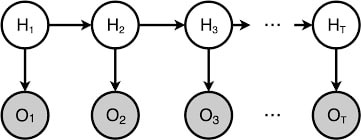
\includegraphics[width=\columnwidth]{images/markovmodel.jpg}
  \caption{markov model}\label{f:markov}
\end{figure} 
The thought process that follows the following explanation is that of a semi-supervised learning. The training data will compose of just words(audio) with their respective speech tag. Also, the training data will comprise a good set of perfectly captioned videos. More than the videos it is the caption files that are important. The individual words file merely provide us with a corpus file of what words to expect. it is the caption files however that allow us to build the Markov model around which the entire caption generation process will be built upon.Now that we have our corpus file we can begin analysis on the caption file to build the model. What we will be doing is using a very simple probabilistic equation\cite{Wikipedia2017a}, The probability of observing a sequence Y =y(0),y(1)....y(L-1) of length of L is given by, \[ P(Y) = \sum_{X}^{} \frac{P(Y/X)}{P(X)} \] . To explain this in a more understandable manner we are looking for relationships between words. For example, when a person is introducing themselves a common sentence is "Hello my name is xyz " or "hello I am xyz". Another assumption we will have to make at this point at least with respect to the current Markov method is that we will work with more complete words that span at least 3 or more syllables so that the model can detect them better. With that, the previous sentences become "hello name xyz" and "hello xyz", from this reduction we can now get a new relationship, two of them in fact. the word hello leads to the follow up of the word name and this leads to the follow up of xyz whatever and hello leads to xyz. Now this relationship will be remembered. Now we can also make use of this concept but towards sentences. First, we will have to determine via some statistical method what would be the best average length [ time duration] for sentences. Now we can use the previous principle to observe if there exist any relationship between sentences and remember them. Now we get on to processing the data to generate the captions. First, we have to eliminate noise from the audio. Then we need to split it into n appropriate sections [ n = total length of video/time of average sentence calculated previously].  Now using MapReduce we can quickly determine how many segments already have a translation [ ie find if there are any perfect/reasonable matches] and obtain the captions for those. If there are none available then we go to the next stage of getting captions word by word. After converting it to a data format appropriately [ this has been discussed this previously in the hearing aid section, another alternative manner will be discussed shortly]. Now we determine the first word, again using map reduce we can match the word to a list of probable similar sounding words. To obtain the actual word the magic of probability comes into play. remember the Markov model we had discussed earlier, from it we can calculate the probabilities of a word occurring as the first word and accordingly make a very educated guess on which word is the right word. Following that using the Markov model once we can determine what the next word could be after first narrowing down the suspects we can use the model to infer what the next word could be. that is, given the current word what is the probability that the next word will be the selected word. \newline
This way we go about generating captions for every word in the sentence. After this is done for all sentences we can generate a caption file for the entire duration of the video. This method is likely to have a lot of errors since the Markov model described here is rather simplistic therefore the onus will have to be on the administrator to go over the captions generated and accordingly make the corrections. This will not only be useful to the people with disabilities but also help improve the accuracy of the system on the whole. Studies have been carried out and more complex implementation of the same idea has been performed with a rather high accuracy rate can be found here \cite{Hakkani-Tur2017}.
\newline
\subsubsection{Automatic caption generation Deep neural network model}
Now the concept of a neural network will be explained. A neural network is based on the on the same idea of how our brains work \cite{wikip[edia2017} . A collection of neurons for information processing and to model the world around us.A very brief explanation would be a neuron sums all the inputs and if the resulting value is higher than a specified threshold it fires. A neural net can be represented as the following figure \ref{f:neuralnet}.

\begin{figure}[!ht]
  \centering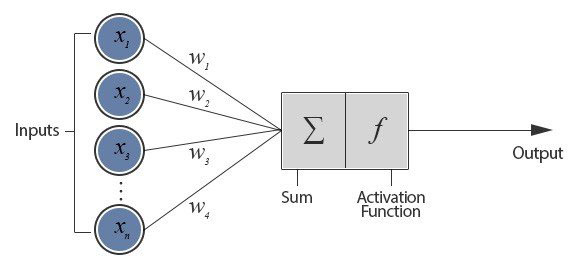
\includegraphics[width=\columnwidth]{images/neuralnet.jpg}
  \caption{neuralnetwork image}\label{f:neuralnet}
\end{figure} 
The above configuration is called a perceptron. It has n inputs and n weights are real numbers and can be positive or negative.The perceptron consists of weights, summation processor and an activation function. the inputs are multiplied by the individual weights and the summation of all of these is passed to an activation function, we will make use of a step activation function which fires 1 if above the threshold a 0 otherwise\cite{wikip[edia2017}. We need to train the perceptron now. This essentially means modifying weights after observing the inputs such that the activation function fires correctly.For all inputs, i, W(i) = W(i) + a*(T-A)*P(i), where a is the learning rate, here, W is the weight vector. P is the input vector. T is the correct output that the perceptron should have known and A is the output given by the perceptron \cite{wikip[edia2017}.When an entire pass through all of the input training vectors is completed without an error, the perceptron has learnt. A deep neural network is thus a collection of perceptrons or to be more accurate it is a multiple layered architectures which compromises of an input and output layer and in between them multiple hidden layers \cite{2017}.[multilayer network image]
From the image we can observe Each input from the input layer is fed up to each node in the hidden layer, and from there to each node on the output layer. We should note that there can be any number of nodes per layer and there are usually multiple hidden layers to pass through before ultimately reaching the output layer.But to prepare this we require a learning calculation which ought to be able to tune not as it were the weights between the output layer and the hidden layer but moreover the weights between the hidden layer and the input layer. Clearly, it becomes obvious that we will need to tune the inputs between the input layer and hidden layer for this we shall make use of a technique called backpropagation which essentially means we carry the error to the next stage of input and then use these errors to modify the input stage of every layer. to be brief we can summarize it as follows We present a training sample to the neural network (initialised with random weights). Compute the output received by calculating activations of each layer and thus calculate the error. Having calculated the error, we readjust the weights (according to the above-mentioned equations) such that the error decreases. We continue the process for all training samples several times until the weights are not changing too much \cite{Pokarna2017}. 
\newline
Now that we have a good understanding of how neural networks work we shall look into how ASR happens via neural networks \cite{Green1999}.we shall go about this step by step. The first problem will be converting sound to bits. We have previously seen digital hearing aids automatically convert sound waves into numerical codes and have extended this concept in multiple places. We shall now go into this a little more in detail and provide an insight into how this could happen. Consider the below wave of sound \ref{f:soundwave}.
\begin{figure}[!ht]
  \centering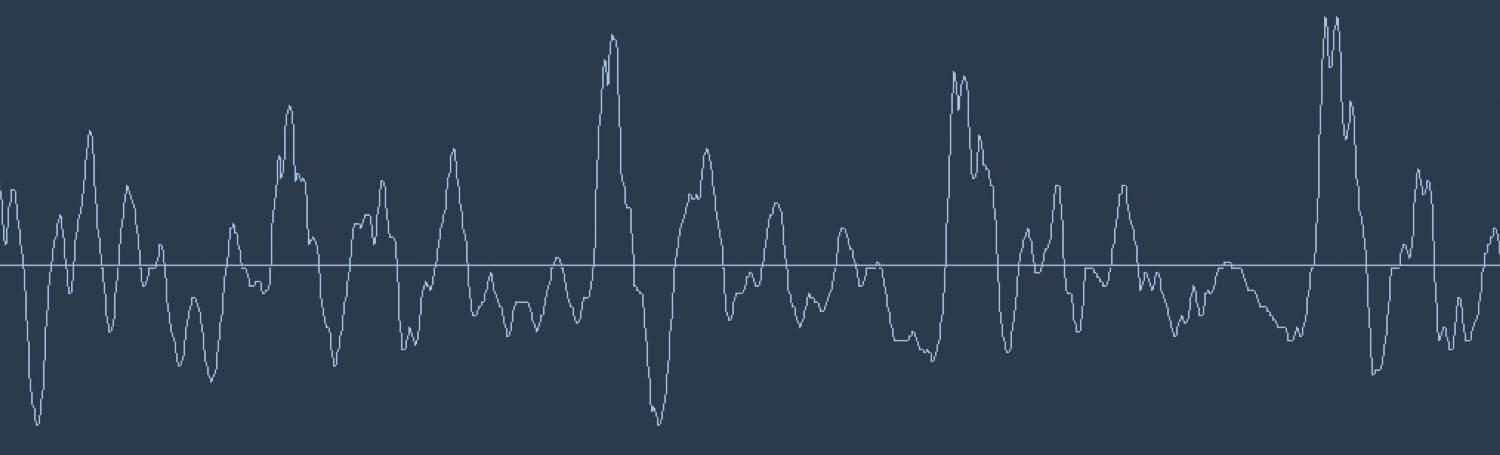
\includegraphics[width=\columnwidth]{images/hellowwave.jpg}
  \caption{soundwave}\label{f:soundwave}
\end{figure}  
This can be represented on a graph as a simple expression of height vs time. The annotations towards height can be amplitude, frequency whatever a person chooses that suits their purpose best. However, note that this is a bit too scattered and not very uniform which is understandable because over digital media the voice can break.Let us attempt to smooth this signal using one of the many transformation algorithms available[ Nyquist theorem for example]. The result will look like this \ref{f:smooth}.
\begin{figure}[!ht]
  \centering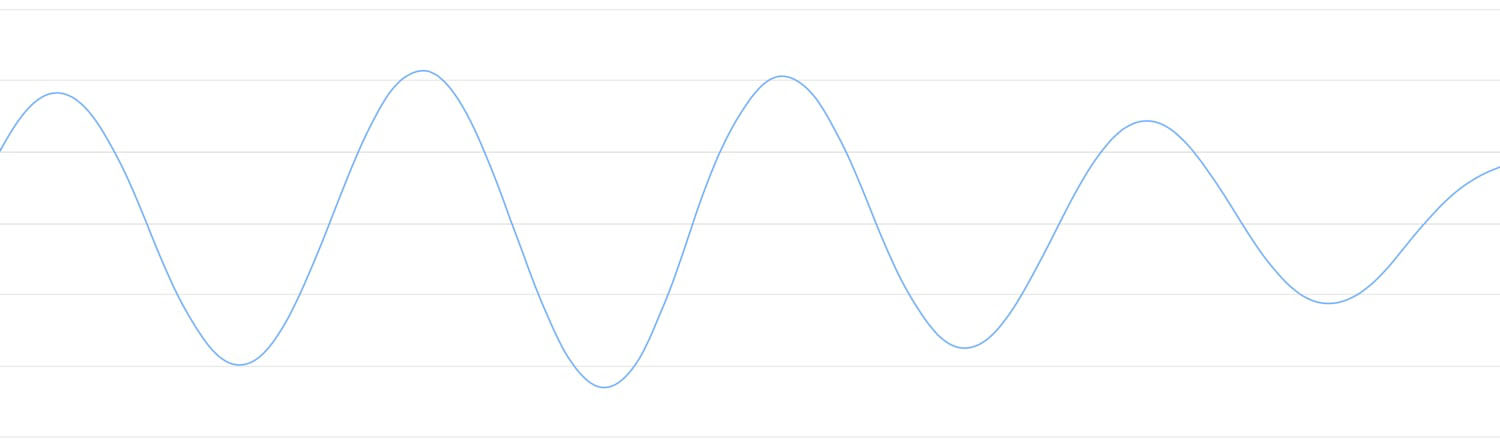
\includegraphics[width=\columnwidth]{images/rephello.jpg}
  \caption{smooth wave}\label{f:smooth}
\end{figure} 
Recall it was mentioned that we can simply take the graph as a function of height vs time, so to help visualize this consider the \ref{f:samplegraph}.
\begin{figure}[!ht]
  \centering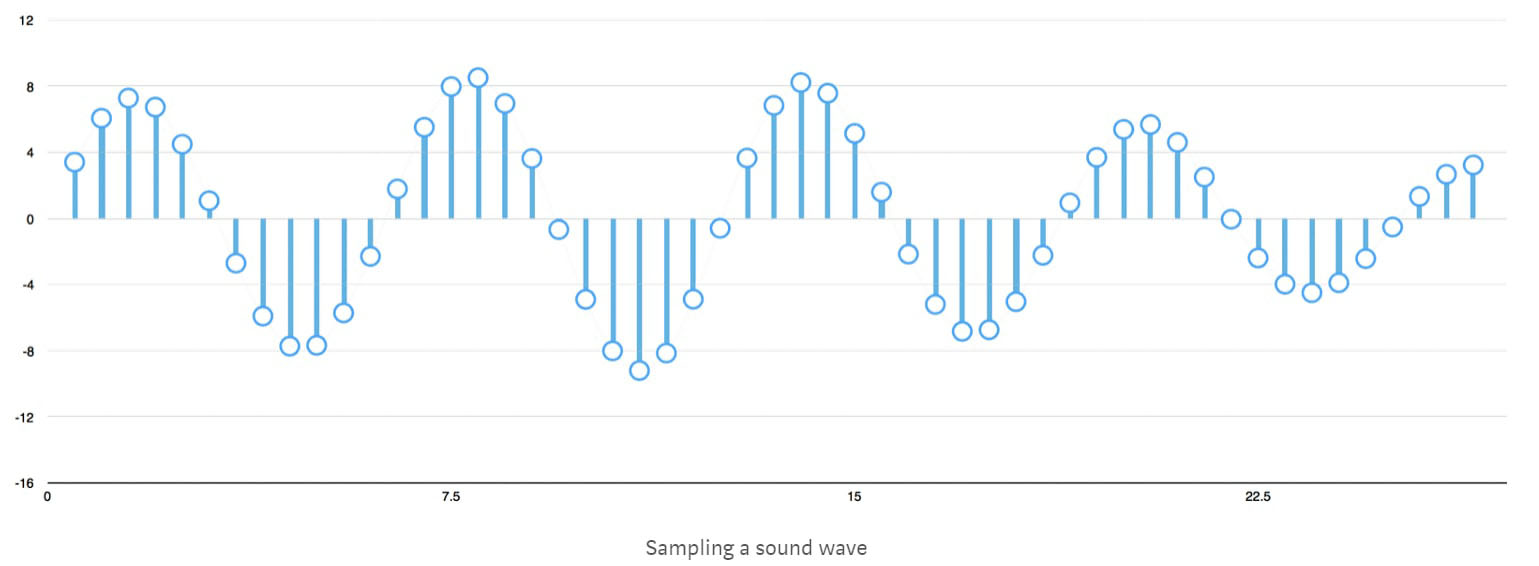
\includegraphics[width=\columnwidth]{images/soundwavesampled.jpg}
  \caption{sampled wave}\label{f:samplegraph}
\end{figure}
To represent this in a text format it would look like [ 100,-20,30,89,789,-400,.....345] where each value is a measure of height over a designated unit of time. We need to be careful about how we select this unit of time. The idea is that different syllables have a different pitch we want to exploit that \cite{2017a} . Hence we want to select a unit of time such that each unit possibly corresponds to one letter. The figure \ref{f:modeloverall}.
\begin{figure}[!ht]
  \centering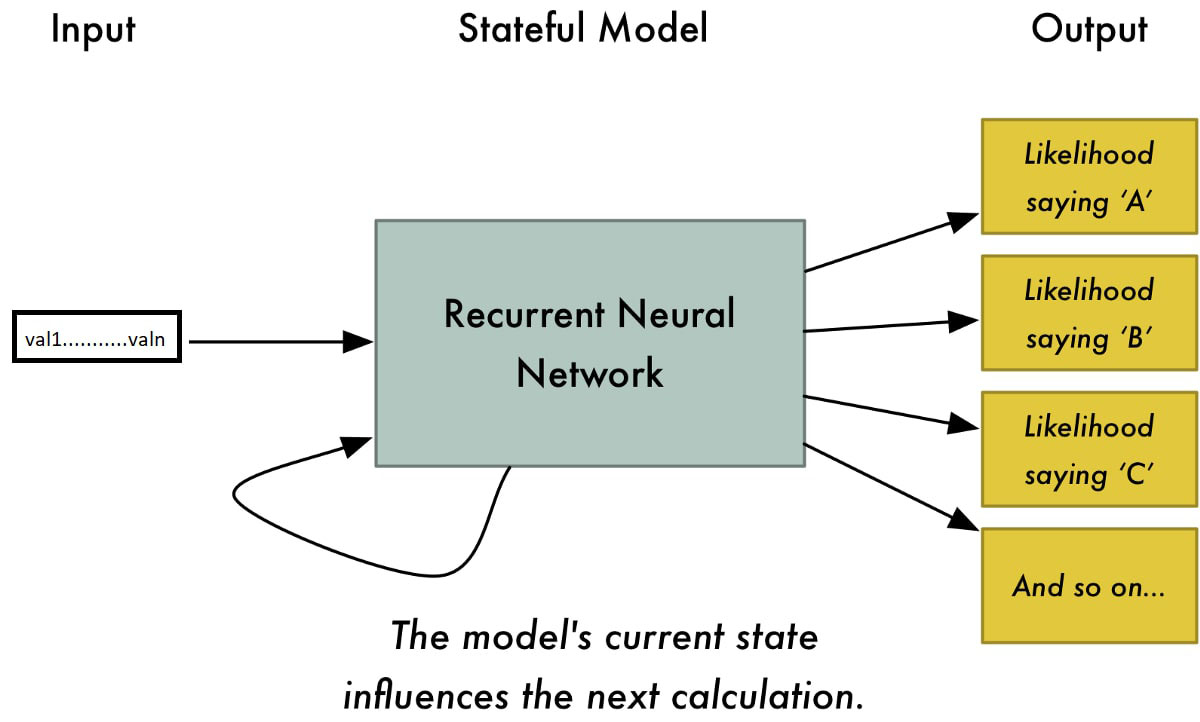
\includegraphics[width=\columnwidth]{images/neuralnetimgsound.jpg}
  \caption{overall neural net model}\label{f:modeloverall}
\end{figure} 
gives an insight into how the overall model should look. So after we have trained the network to recognize each letter based on value/set of values we proceed with feeding the current input stream and thereby obtaining each letter. We can then pair these letters to form a word. Note that there is a high chance that many letters could be repeated, decisions must be made based on observations if we need to replace repetitions. Once we have obtained these words there is a possibility of spelling errors using an auto-correct program [there are many good algorithms available on the internet] we can then use the Markov model we previously explored to verify its correctness [ if the word generated fits the model observed]. To save some time we could use map-reduce again to find out if similar patterns exist before and then use it accordingly to determine if there were similar instances before.

\subsubsection{Using Image Processing to generate captions}

It is well known how powerful OCR is it can convert text images into a text file by "reading". What if we could apply a similar concept when people are speaking. People who have hearing disabilities especially those who have severe hearing disabilities and cannot always make use of sign language to get by make use of lip reading. Lip reading has existed for a long time and there is no particular skill or technique about it. People familiarize themselves with the movements of the lips with respect to different sounds and then make use of that pattern. We will not go too deep into the specifics of how to process features and use them to recognise these patterns, we have already exhaustively covered neural networks and Markov models in great detail. Depending on how the features were extracted and stored learning can occur. We shall instead focus on the process of obtaining the images for processing the features.Since we are going to be focusing on extracting the facial features we need a device that can focus on the face. Two devices that could be used are the smartphones and perhaps a not so popular option in google glass. Both devices have powerful cameras with which pictures can be taken. Note that captions generated will be with some delay. Converting these devices into IoT devices shouldn't be particularly hard. Using map reduce we can effectively store these images and in a quick manner, to save data however we could probably convert the image into an rgb matrix text file and send. Map reduce plays a very very important role here, rather than sending the same image again and again if a mapping is found to exist already we can make use of it. To extract features OpenCV has a great library that could aid in the feature extraction making use of these features for processing depends on the implementation. Note that big data here if a good bunch of people are observing the same thing, like for example watching a news broadcast, seminar etc. We can use a combination of big data and IOT to determine these similar users and make one person the central hub, he/she will process while the results are shared between all or alternatively each person can send sections at regular intervals to reduce the processing time. For example, if 4 persons are detected person each person can do 10 seconds order depending on implementation this should help keep the process more real time. Note that however, this would be very situational but in situations where transcripts are not made available and the environment is way too noisy for a speech to text caption system to be implemented this comes very handy. While we are on the topic of using these devices as IoT a future possible implementation, especially for smart TVs, would be to do detect such devices and send the subtitles to the device. Too many times if watching from a  distance subtitles from a distance a person am not be able to read them having it sent n the device would mean the person can see the tv and read comfortably especially in the case of google glass.

\subsubsection{Captions for the blind and deaf}
It has been covered in detail how we can go about to help those who are hard of hearing. But there are many people who are both deaf and blind. It is appropriate that we consider the difficulties these people face too and think of a possible solution. All considered one of the most important thing blind and deaf people would need is a braille machine ( provided they know braille). There exists technologies that create Braille on the fly and are IoT supported. Combining all of the previous discussed technologies with this wont be particularly hard the only note able difference is instead of outputting captions they need to be converted to a braille format instead.

\subsection{Data Processing and Technologies}

Data processing has been covered in advance very well in the previous sections. For those who are unable to build a custom neural network or are struggling to implement it can make use of the Watson API. Watson was created as a question answering (QA) computing system that IBM built to apply advanced natural language processing, information retrieval, knowledge representation, automated reasoning, and machine learning technologies to the field of open domain question answering. When created, IBM stated that, "more than 100 different techniques are used to analyze natural language, identify sources, find and generate hypotheses, find and score evidence, and merge and rank hypotheses."In recent years, the Watson capabilities have been extended and the way in which Watson works has been changed to take advantage of new deployment models (Watson on IBM Cloud) and evolved machine learning capabilities and optimized hardware available to developers and researchers. It is no longer purely a question answering (QA) computing system designed from Q\&A pairs but can now 'see', 'hear', 'read', 'talk', 'taste', 'understand', 'reason', 'interpret', 'learn' and 'recommend' \cite{Wkipedia2017ibm} . This article \cite{Massachi2017} provides a very good explanation on how to use the watson API to generate captions.

\subsection{Section conclusion}
Captions are a very important methods of understanding conversations and proceedings. with advancements being made it AI the challenge is now geared towards generating captions with 100\% accuracy. Players both big and small are starting to take up the process of caption generation more seriously. Aside from helping people who are hard of hearing caption generation is important because of its other uses , it can overcome the language barrier and become a very powerful tools for envoys possibly removing the need for interpreters. There should be more funding and activity from the government over this issue. Getting captions most of the time is not easy and the current guidelines are reactive rather than proactive. Technologies exist , personnel exist , motivation for doing such helpful work is at an all time high all that is needed is a little push. On the technical front as mentioned all the big tech giants are actively focusing on AI but they all are looking at the bigger picture. AI to perform tasks on the whole. there is always a chance for smaller corps to pick up small important pieces of detail that could really make a difference. for example, the google glass project has not really made much progress and caption generation is not their priority. However, companies exist who have made facial expressions to captions a reality on devices like smart phones. Someone could put two and two together and make a device that costs lesser than a hearing but delivers the same impact.

\section{Big Data and Noise pollution}

\subsection{Introduction}
Every day, we experience sounds in our environment, such as the sounds from television and radio, household appliances, and traffic. Normally, these sounds are at safe levels that don’t damage our hearing. But sounds can be harmful when they are too loud, even for a brief time, or when they are both loud and long-lasting. These sounds can damage sensitive structures in the inner ear and cause noise-induced hearing loss (NIHL).NIHL can be immediate or it can take a long time to be noticeable \cite{NIDCD2017} . It can be temporary or permanent, and it can affect one ear or both ears. Based on a 2011-2012 CDC study involving hearing tests and interviews with participants, at least 10 million adults (6 percent) in the U.S. under age 70—and perhaps as many as 40 million adults (24 percent)—have features of their hearing test that suggest hearing loss in one or both ears from exposure to loud noise \cite{NIDCD2017}.Loud noises like explosions, repeated exposure to loud music for extended periods of time are few of the factors that lead to NIHL.Sound is measured in units called decibels. Sounds of less than 75 decibels, even after long exposure, are unlikely to cause hearing loss. However, long or repeated exposure to sounds at or above 85 decibels can cause hearing loss. The louder the sound, the shorter the amount of time it takes for NIHL to happen.

\subsection{Big data and how to tackle noise pollution}

So far a very reactive approach was taken towards tackling hearing loss and while they all are good approaches as the saying goes prevention is better than cure.Now we shall take a look at how integrating big data with the IoT devices we have at hand can go towards helping us curb NIHL. The device is none other than the mobile phone. The mobile phone is one of the pinnacle devices that leads the IoT trend. The fact it has the high processing power and can access the internet almost anytime allow for many desirable solutions. So how do we go about tackling this problem, quite straightforwardly it is a good practice to avoid sources of loud sounds. How can we do this, two ways one we can proactively scourge the internet and google maps for situations like traffic, construction sites and other such noise pollutants and then analysing these chart routes to avoid them. This works well only if we have such data available via maps, internet. The other way is to use the same implementation of the previous but rather than depending on internet and maps have people update this information via an API. One more possible implementation is to use the speakers on the phone and use it as a sensor and then use GPS data to accordingly update information. If the majority of the public agrees to this then the amount of data will be humongous and definitely big data technologies like Hadoop, pig, hive will be required to store efficiently but this method will have loads of data charges and will be a drain on the battery life. It could help if governments could fund for specific IoT devices that listen to crucial junctions like signals that the government and or public could use. This way the governments could have a portal maintained by them that actually suggests places of high noise pollutions. The added benefit to this is that the government can monitor round the clock violators of noise pollution and can proactively set out to catch these offenders.
\newline
While the above may/may not be implemented yet one way we can protect ourselves is by using ear plugs, But the most common complaint would then be that of boredom and discomfort. Most head and earphone companies these days make use of excellent noise cancellation technology. We can use big data and mobile phones to play music that is at the opposite frequency of the sound to cancel out such unwarranted noise. Aside from external noise we now must consider how harmful is the music we listen to. Music has evolved the music of these days have evolved from peaceful melodies to high-intensity powerful tunes. More often than not we get lost in the euphoria of these tunes and subconsciously increase the volume to maximize the effect of this rush. Using big data we can control these habits via big data we can dynamically analyse which songs are most likely to cause such situations by looking at the loudness distribution fo the music and then collectively comparing the instances when other people suddenly increase their volumes. note that no one can dictate a person what to do unless they have explicitly given permission settings to do so. What we can do is whenever a person suddenly increases the volume that way past a safe threshold we ca display warning messages that will alert the user that he/she is at risk of damaging their eardrums.

\subsection{Section Conclusion}
There are many unique possible solutions to counter the problem of NIHL. Ultimately both the government and its people need to be proactive and neither should wait for the other to make the first move. Governments need to start creating more awareness about the effects of NIHL and need to start funding research into tracking NIHL digitally if they do not have the required personnel to track manually. With everything going digital ultimately this implementation will have to happen somewhere down the line. However the sooner they get a start to it the sooner this problem can be curbed. people too can be proactive about this and try to keep their environment as sound friendly as possible. noise cancellation technology at the minute is rather limited towards to just ear and headphones but if the current noise pollution level trends continue it wont be long before we look at buildings being built with a mandatory soundproofing scheme.

\section{Big Data and hearing loss, Medical}

\subsection{Introduction}
Hearing loss can occur due to a myriad of medical reasons from colds to trauma to accidents. While a lot of these don't have facets where we can apply big data to reduce the probability of hearing loss occurring Big data can help in identifying the early symptoms of these problems and suggest preventive actions. The first-way and most hearing loss can occur due to medical reasons is that of the common cold. When we contradict a common cold the ear nose and throat being interconnected the infection spreads everywhere. this infection causes a buildup of fluid in the middle ear, making it difficult for sounds to travel efficiently from the outer ear to the eardrum. Individuals may notice a clicking sound in their ear or that conversations and noises are muffled. The congestion may also lead to an ear infection, caused by bacteria or a virus in the middle ear, and lead to temporary hearing loss \cite{Wikipedia2017}. The other factor that that leads to hearing loss is the disease meningitis. Meningitis is an inflammation of the membranes (meninges) surrounding your brain and spinal cord.The swelling from meningitis typically triggers symptoms such as a headache, fever and a stiff neck \cite{mayoclinic2017}. Studies have shown how dangerous meningitis in particular bacterial meningitis is towards causing hearing loss \cite{mayoclinic2017}.The cause for the hearing loss enters the realm of biology, but the article \cite{Richardson1997} states that meningitis leads to lesions developed in the meninges layer and causes neurological damage. The next cause of hearing loss we shall look at is that caused due to trauma to the head due to accidents.

\subsection{Applying Big data}
It should be noted that leading a healthy lifestyle to prevent illness is an onus that should remain on the person, There are very detailed national registries that provide checklists of which vaccines to take and when. The prerogative thus remains on the person to be healthy and vaccinated. That being said using big data and IoT one can track their everyday activities and then use these details to compare it to a centralized plan and modify their activities. plenty of such apps exist but they are not entirely smart as they require manual input but are a good start. Improvements in terms of implementations of IoT devices to track such changes would be very useful. We can make use of these features to lead a healthier lifestyle and build more robust immune systems a natural way. Aside from this we also would able to track any sudden changes in our health, if we suddenly show symptoms of a cold etc the change in regular pattern would be detected, a cold could lead to body temperature to increase , lethargy, etc these changes could be compared to people with similar fluctuations and then a plan for corrective action could be suggested this is very much like looking up your symptoms online through a portal like WebMD only that you now have data to back it up. Also, this data could be very vital to when you visit a doctor as a doctor could analyse these logs and they could provide a more detailed information than the normal guesswork of replies the doctor would normally receive. A lot of research has been done in detecting diseases like meningitis using big data however this enters the realm of biology and is another paper in its own right. We instead shall focus on analysing MRI images to detect anomalies that could be caused by diseases like meningitis. Note that we would be able to just detect anomalies but there is a high chance these anomalies could be just noise. The purpose of using big data is to minimize the risk of being misdiagnosed as treatments for meningitis could cause more harm if misdiagnosed. Ultimately it is safer to get a second opinion and treat the analysis provided by the big data with a pinch of salt.
\newline
Safety of an individual ultimately lies in their own hands, discounting factors such as bad luck and freak accidents things that cannot be controlled.Also, note there is nothing much that can be done in the event of an accident occurring other can call paramedics, it more risky to make the situation worse by performing actions that could be detrimental to the situation it is best to remain calm and wait for help and follow very basic first aid practices. That being said big data can be sued to help the respective authorities reach and react faster to accidents and lessen the damage trauma can cause. IoT devices installed in accident prone/ busy zones can be trained to detect crashes. When a crash occurs it can be used to notify the nearest hospital with enough available resources. So we are looking at an implementation of having data of all hospitals in a region and their available resources by this we mean available ambulances ready for use and perhaps logistics like available trauma specialists and the like, this way people in distress won't have to wait too long for medical attention and everyone is covered better. Aside from separate IoT devices personal devices like mobile phones, wrist health meters can be trained to detect sudden changes in the body like falling blood pressure, etc and alert the user if the user doesn't respond then the device alerts the nearest hospital. A specialist in the hospital can monitor these details to decide if this is due to negligence or a person is actually in distress.

\subsection{Section Conclusion}
Big data has a lot of applications in the field of medicine, but the motivation to stay healthy should come from the persons themselves. There is a lot of research happening in the field of medicine to make the process of getting a diagnosis at least a lot cheaper than the current rates. But these diagnoses always should be taken with a  pinch of salt. most programs only look at what is in front of them and may not be able to determine relationships between different diseases, they may however at least bring to attention potential anomalies which may have been missed and suggest a second opinion may be a good idea. In terms of hearing loss and medical big data cannot yet play a big part, once more co-relations have been made between data and meningitis detection it will have to be limited towards potential MRI detection, but by no means is this a small feat MRI is very costly and big data may reduce the need to undergo multiple MRIs as it could help it confirming the presence of anomalies or rule them out altogether. The same can be said of trauma prevention. Big data can be merely sued to make sure help is received sooner. It can be used as a preventive measure to make sure people don't use accident-prone routes etc.

\section{Conclusion}
Hearing loss is a problem and once upon a time it could be considered creating a liability on the society, however, the application of big data and emerging technologies could help turn this liability into something positive. It certainly is creating a lot of job opportunities for one. there are multiple new startups created to develop on facets like speech to text conversion via a mobile phone, big players are trying to reach overall 100\% accuracy. people affected by hearing disabilities now find themselves with much more options than before and also have opportunities to contribute and be a part of something big. Another positive is that the application of big data is providing a paradigm shift and is now creating more new kinds of hearing aids each of which incorporates more and more powerful features. it may not be too soon before this hearing aids down the line become new "smart earphones". Caption generation has a huge potential market too but it is only the big players who are making significant headlines. The race for 100\% is wide open and anyone stands a chance to make a name for themselves. The current set of government policies and funding are more that of a reactive than proactive approach changes can help drive research and also create new jobs to make resources available everywhere for anyone to use. Big data has a lot of applications is healthcare which is constantly evolving there will always be new avenues to apply big data, it is, however, a risky move because any misdiagnosis or wrong suggestion could lead to fatalities which could lead to lawsuits. The benefits, however, outweigh the risks and most patients are smart enough to know that predictions from a computer are to be used as a reference and not the rule.



\begin{acks}

  The authors would like to thank Dr. Gregor von Laszewski for his support and suggestions to write this paper.

\end{acks}

\bibliographystyle{ACM-Reference-Format}
\bibliography{report} 


\end{document}
